
\vspace{-10ex}%
\rule{\textwidth}{0.3pt}
\vspace{5ex}
 % after-code

\textit{
A deeper look into each component with some information of their functionality and implementation will be presented in this chapter. Why some specific components are chosen is also answered here. 
}
\vspace{5ex}

%\gls{usb}\gls{ti}\gls{via} \gls{adc}\gls{cad}\gls{drc}\gls{erc} 
%\gls{ptc}\gls{png}\gls{lga}\gls{gpio} \gls{led}\gls{jtag}\gls{pwb}\gls{erc}
%\cite{si4460}

\section{Layout parameters}

When starting the layout some initial rules need to be set up. These parameters are set by the board manufacturer.
The design can be produced at different places but when ordering from this manufacturer the constraints that are used is the same parameters that the supplier uses as their standard.
These rules and constraints may differ from one supplier to another but as the company already this supplier the same will be used for this project.
Naturally, for this project, the minimum spaces and distances that does not make for a supplement charge are chosen as the design rules. A list of these parameters can be seen below.

\begin{itemize}
\item Trace width: minimum of 6 mils (0,1524mm) 
\item Via diameter: 10 mils
\item Maximium thickness of board

\end{itemize}
 
\subsection{Landgrid}
%The industry standard is always good to aim for, in this case, the basic designs are taken from \gls{ipcg}'s design guidline\cite{ipcg}. While these are made for optimal manufacturability the footprints used on the test board are modified to enable for easier solderability, production and rework if needed. The land grids are made slightly bigger and longer to achieve this. The downside of making the pads larger is that the final board size increases and therefore the size of the land grids require to be reduced.

\subsection{Easy prototyping}
The components that are going to be used in high frequency often come in tiny packages. This gives the protypability problems with easy ability to solder and use, but the problem is that the best components used in this area of work will be small to fit in small advanced systems. To make a

\section{Structure}
The product is constructed with a number of components, which all have a central role in the final product. They can all be seen in \autoref{fig:sys_dia}. A list of the major components and their function can be seen below:

\begin{itemize}[noitemsep] 
\item \gls{mcu}: The central part of an integrated system, handles all the calculations and the program code.
\item Radio: All the communications with the rest of the world will be handled by the radio, sending on the VHF and UHF band.
\item \gls{imu}: Movement detection is measured with an accelerometer, this to determine if the unit is in motion or lying still. 
\item \gls{ldo}: A Low-dropout regulator can supply the system with a smoother voltage because no switching is taking place.
\item Hall sensor: The hall sensor is used as a switch for the system by sensing if a magnet is nearby and then turning off the circuit.
\item \gls{rtc}: A real-time clock is important to acquire data at a specific set time. It is important that the clock is exact over the whole life of the product.
\end{itemize} 


\begin{figure}[H] 
	\centering 
	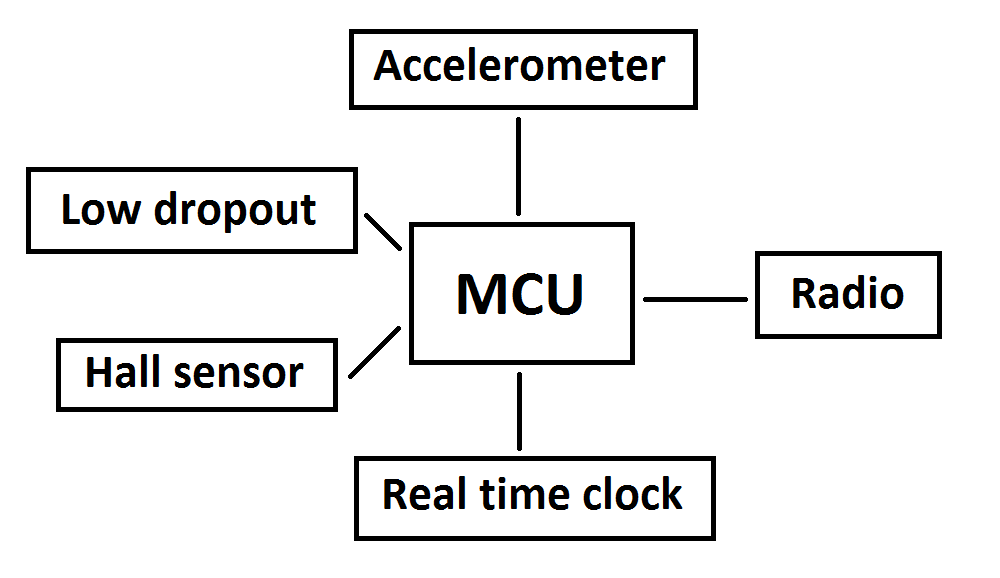
\includegraphics[width=.8\linewidth]{Figures/System_diagram} 
	\captionsource{The prototype connection}{Aurthor}
	\label{fig:sys_dia} 
\end{figure} 

Each of the components of this project is carefully chosen to get the functionality and effect that the company is after. To ensure the system works as intended the company has acquired development boards to each of the components. Every component needs to be tested to ensure their individual functionality. Each development board is connected to the microcontrollers board. First off, the \gls{mcu} have to be set up in a correct way with all its parameters and then the other components could be connected and initialized one after another. The whole connection can be seen. %\autoref{rattbo}.

%\begin{figure}[H] 
%\centering 
%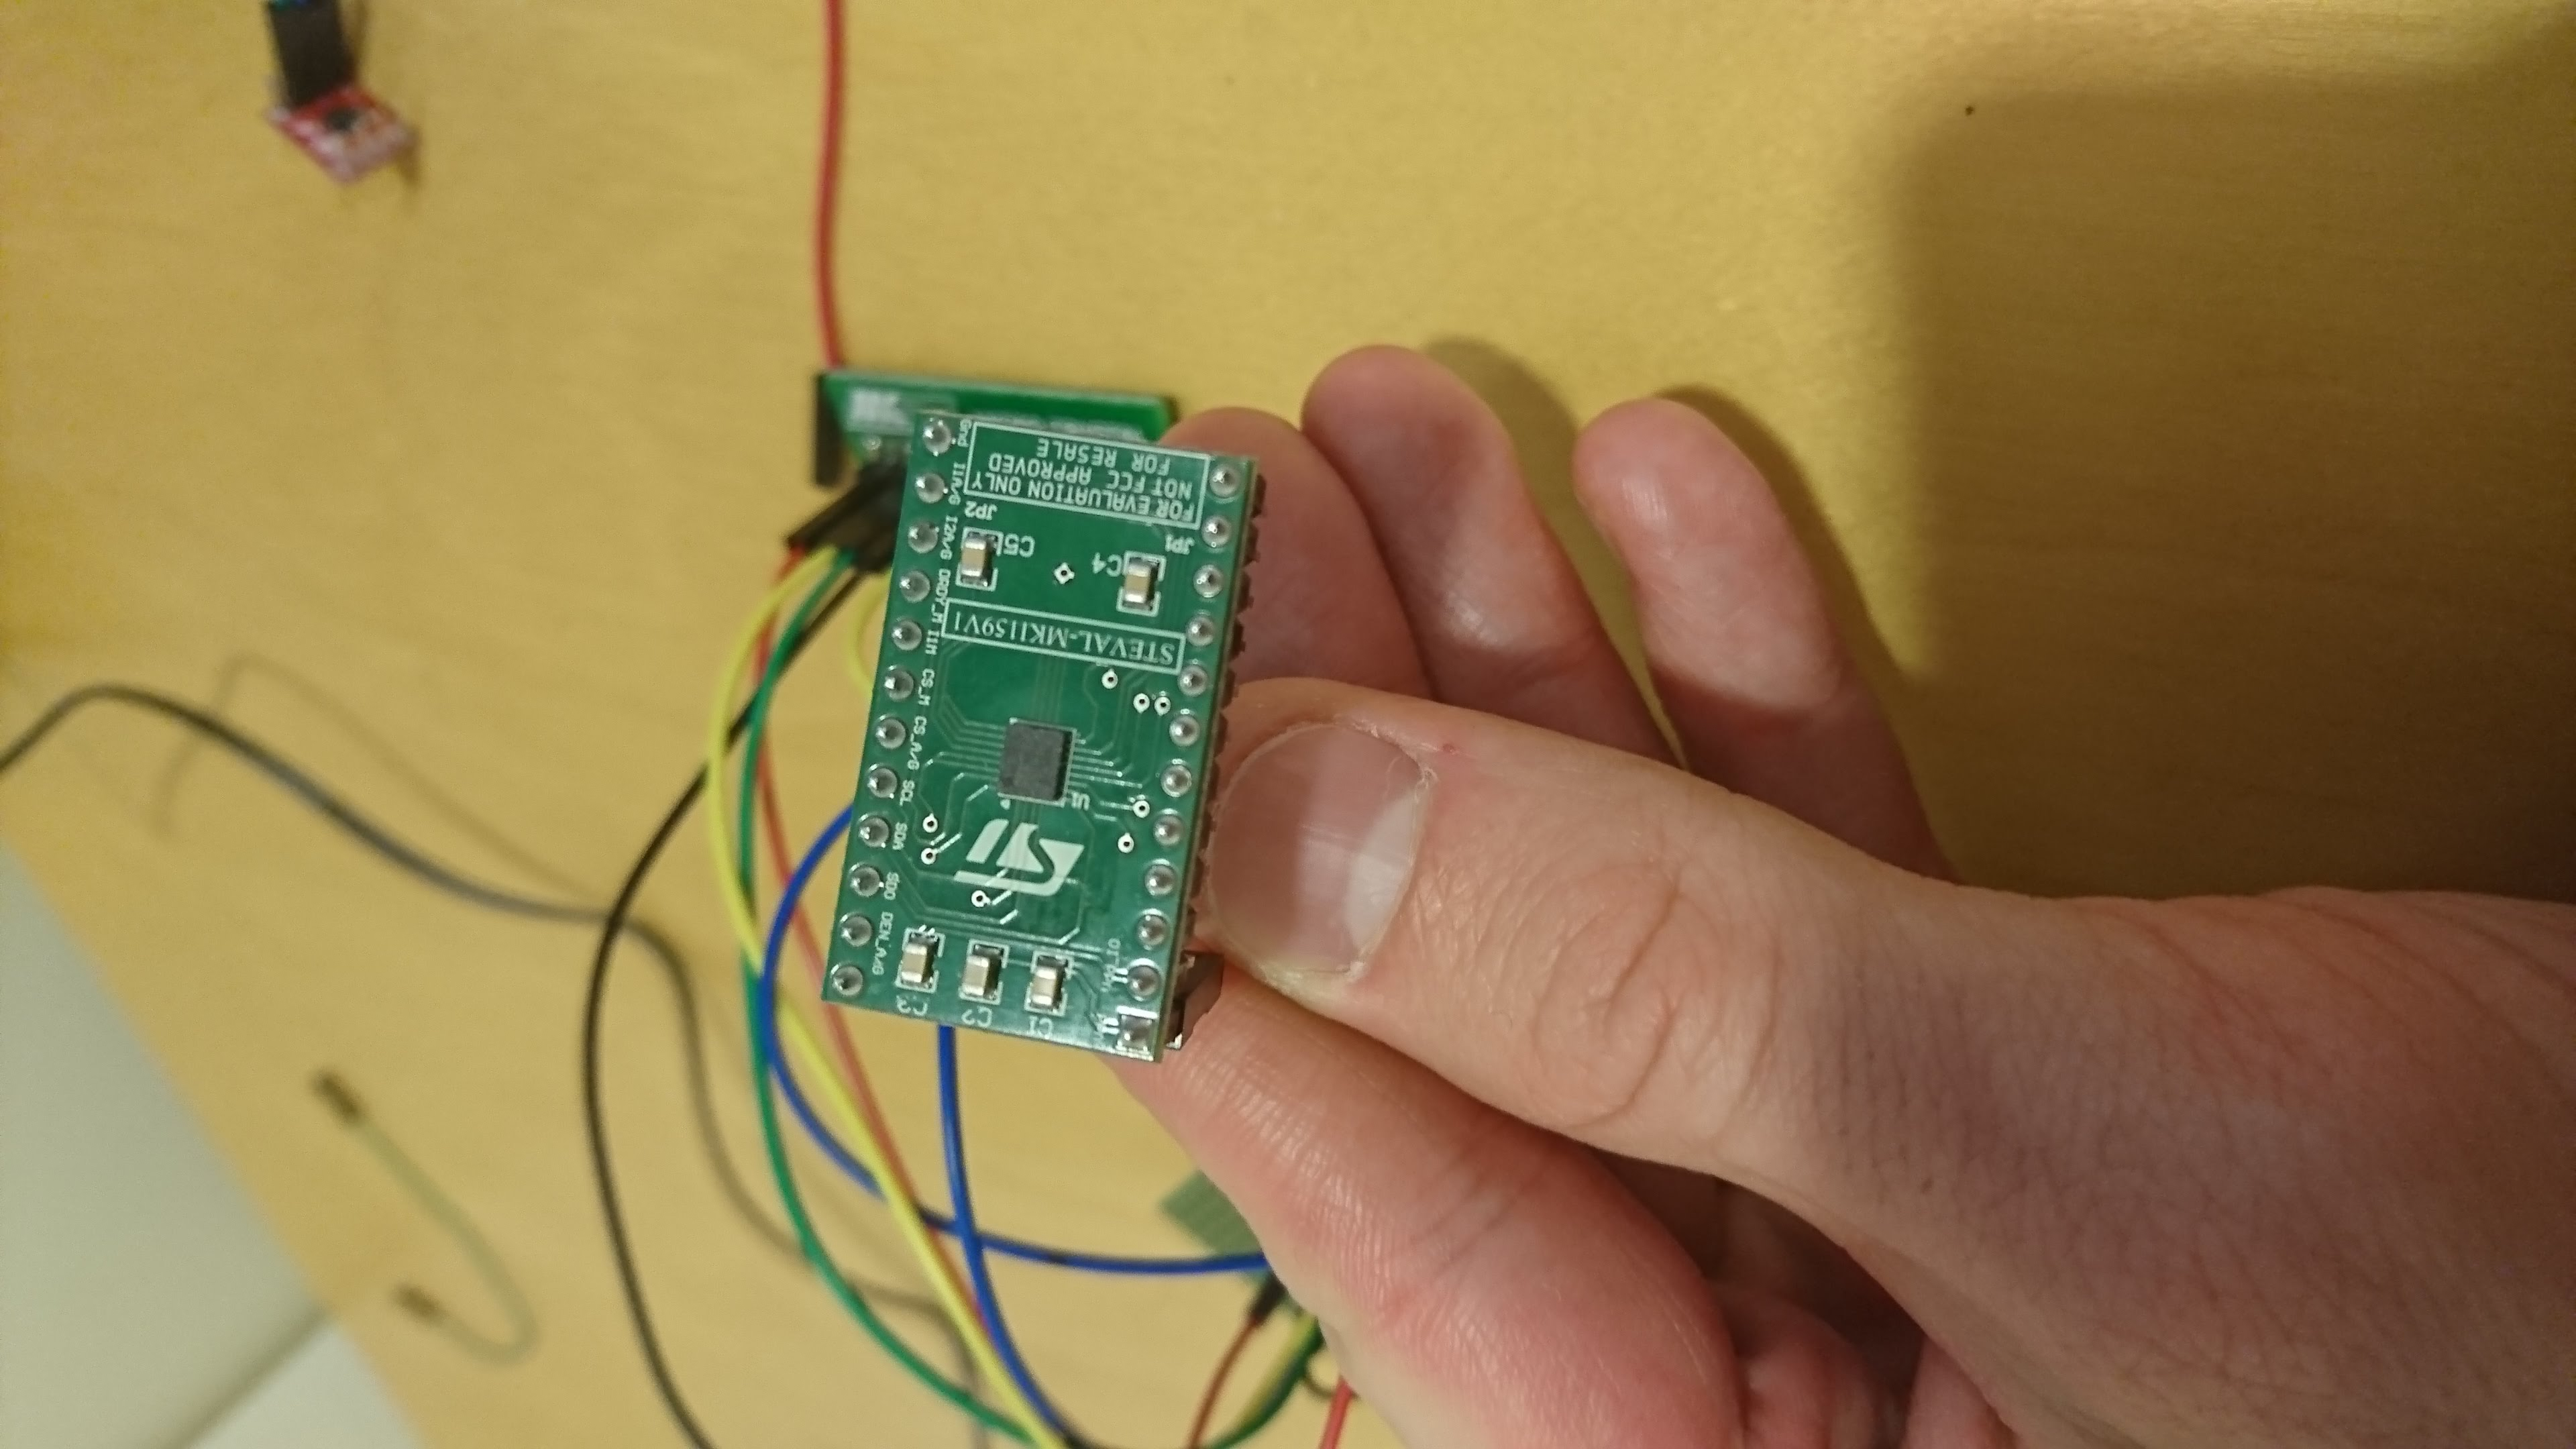
\includegraphics[width=.8\linewidth]{Figures/DSC_0103} 
%\captionsource{The prototype connection}{\url{Aurthor}}
%\label{rattbo} 
%\end{figure} 

%The \gls{mcu} can dtad


\section{MicroController Unit}
The \gls{mcu} used for this project is a processor type that is used by this company many times before and has been chosen to this project for its small size, low power draw, sufficient connections, and features. The particular processor used is the PIC18LF46K22\cite{pic18}. The version used is one with 40 pins. All the connections available are shown in \autoref{Pic18_Pinout}.

\begin{figure}[H] 
\centering 
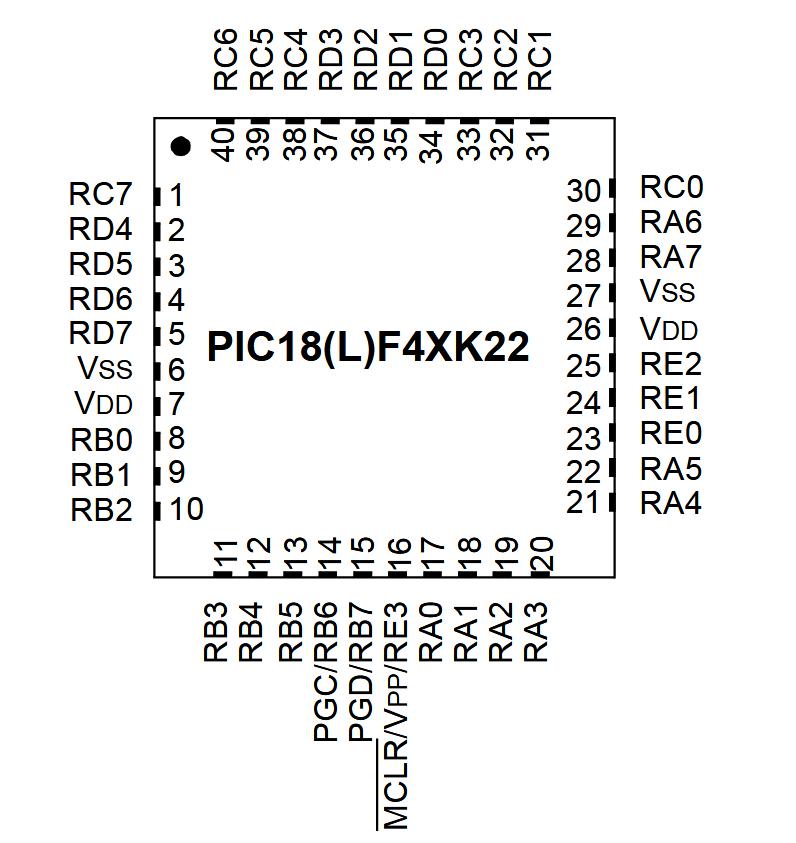
\includegraphics[width=.7\linewidth]{Figures/Pic18_pinout} 
\captionsource{PIC18LF46K22 pinout}{\url{http://ww1.microchip.com/downloads/en/DeviceDoc/40001412G.pdf}}
\label{Pic18_Pinout} 
\end{figure} 

\subsection{Connenctions}

 \subsection{Power}
Powering it is done by connecting the VDD pins to the power net. Connected to the ground is the Vss pins on the processor. To ensure the current fed is as smooth as possible capacitors are connected between these two pins. The value of these capacitors is chosen to 100nF.  

\subsection{Oscillator}
To operate the \gls{mcu} a clock signal is mandatory, this can be implemented in different ways. Either with the internal High, Medium and Low-frequency oscillator or an external one. Where the external rely on a specific circuitry to provide the clock source. Examples of external oscillators are clock modules, quartz crystal resonators or ceramic resonators and resistor-capacitor circuits. When a circuit is specified to be power efficient the speed of the clock plays a central role. As this product is specified to run on a small battery the speed of the system is kept low to increase the lifetime of the battery. The clock signal is generated from an external temperature compensated Crystal Oscillator (TCXO).


\section{IMU}
The motions of the system is measured with an IMU system. This system can be used in a lot of different cases, both to detect if the unit is stationary or moving or if there is very hard and fast movements in the product. One of the simplest IMU's is the 3-axis accelerometer, it

\newpage
\section{Accelerometer} %% Accelerometers
The component used is a 3-axis, ultra-low-power and high-performance accelerometer from ST \cite{ST_acc}. The component is the simplest of IMU's that this manufacturer has and this simplicity makes for a product that is only incorporate one single function. 3-axis accelerometer means that it can measure 

\section{Power}
Two voltage connections are apparent on this device, one which is called VDD and the other is called VDD-IO. The VDD is the supply voltage and VDD-IO determines the logic voltage level. 

\subsection{Connenctions}


\subsection{Software implementation}



\newpage
\section{Radio}


\subsection{Power}


\subsection{Connenctions}
 In the registers 


\subsection{Solidworks PCB}
Followit uses the PCB board design software Solidworks PCB from DASSAULT SYSTÈMES. It utilizes the industry-proven Altium design engine for layout and routing of printed circuit boards and combined with a close connection with the mechanical CAD of classical Solidworks. With this program, the PCB layout and design can be transferred seamlessly over to the mechanical environment to create an exact case or enclosure for the circuit board. The version used in this thesis is (Update 2.0).


\section{Power consumption}
 The total power consumption is calculated by adding the current draw from each individual component together.  A different test is conducted to try different modes of the system. One describing the power consumption of only the processor. This is done by running it in an infinite loop with all the other components at the circuit powered down or in power down mode. Since the system is not supposed to be active just a small time with a longer power down mode in between the power consumption on the system has to account for a longer time span. The tests are made with a standard scheme used already by the company. The scheme consists of a small radio pulse every second and the system being inactive in between these radio pulses. 
All the systems 
